\documentclass[12pt]{article}

\usepackage[margin=1in]{geometry} 
\usepackage{amsmath,amsthm,amssymb}
\usepackage[spanish]{babel}
\usepackage[utf8]{inputenc}
\usepackage{tikz-cd}
\usepackage{amsmath}
\usepackage[shortlabels]{enumitem}
\usepackage{mathtools}
\usepackage{float}

\title{SWAP: Práctica 2}
\author{
        Antonio Gámiz Delgado
}

\begin{document}
\maketitle

Primero habilitamos la sesión por \textit{ssh} sin contraseña de \textbf{M2} a \textbf{M1} (y viceversa):

\begin{figure}[H]
   \center
  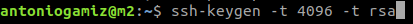
\includegraphics[scale=0.5]{img/_1.png}\\
  
\includegraphics[scale=0.5]{img/_2.png}\\
  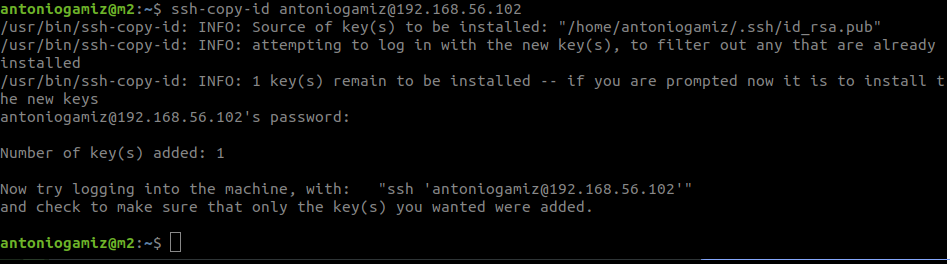
\includegraphics[scale=0.5]{img/1.png}
\end{figure}

Instalamos \textit{rsync} (aunque ya estaba instalado):

\begin{figure}[H]
   \center
  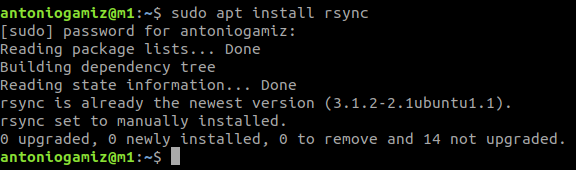
\includegraphics[scale=0.5]{img/2.png}
\end{figure}

Cambiamos el \textit{owner} del directorio \textit{/var/www}:

\begin{figure}[H]
   \center
  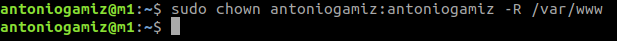
\includegraphics[scale=0.5]{img/3.png}
\end{figure}

Comprobamos el correcto funcionamiento de \textit{rsync} copiando el directorio \textit{/var/www} (desde \textbf{M2}):

\begin{figure}[H]
   \center
  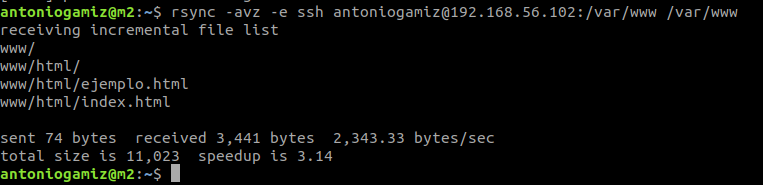
\includegraphics[scale=0.5]{img/4.png}
\end{figure}

Modificamos el archivo \textit{/etc/crontab} y añadimos la tarea para hacer sincronizar el directorio \textit{/var/www}:

\begin{figure}[H]
   \center
  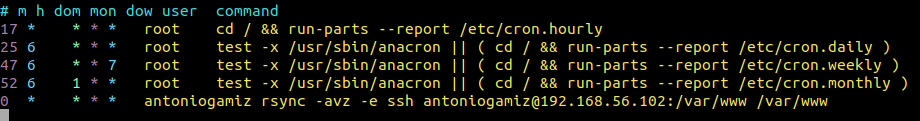
\includegraphics[scale=0.5]{img/6.png}
\end{figure}

\end{document}